% !TEX root = ../main.tex

\chapter{Presentation of the company} % (fold)
\label{chp:presentation}

\section{The company} % (fold)
\label{sec:company}

Algolia~\cite{algolia-home} is a company founded in Paris, but now has its headquarters in San Francisco, US, although most of the development happens in Paris. Their goal is to help people discover content they want to find, which is achieved by a SaaS search offering.

People upload their data onto Algolia's infrastructure, where the data is split up into n-grams~\cite{kimbrell1988searching}~. Using n-grams results in creating a nested data structure that’s very fast to search in and has features like typo-tolerance, faceting etc.\ at  the cost of a slightly higher indexing time (a few seconds to a minute).\cite{paris-nlp-algolia}

The story doesn't end there, because developer experience (DX) is held in a very high standard at Algolia. There are API clients for a lot of languages~\cite{doc-api-clients}~. In JavaScript and mobile the offering goes further than that, by offering what’s called InstantSearch~\cite{instantsearch-js, react-instantsearch, instantsearch-android, instantsearch-ios}~. These are a set of libraries orchestrating all parts of a good search experience.

\begin{figure}[H]
  \centering
  \includegraphics[width=0.5\textwidth]{../assets/algolia-logo-light.pdf}
  \caption{The logo of Algolia~\cite{algolia-press}}
  \label{figure:company-logo}
\end{figure}

\section{Work environment}
\label{sec:work-environment}

Algolia is divided into several ``squads''. According to an internal handbook an Algolia squad is

\begin{quotation}
  a group of people working on projects that are alike. A squad involves people with different skillsets, profiles \& backgrounds
\end{quotation}

The squads that Algolia currently has in the engineering department are:

\begin{description}
  \item[Acquire] public website development and the landing pages
  \item[Core] the search engine and the web dashboard
  \item[Empowerment] development of all libraries (except API clients) and helpers to make integrating Algolia smoother
  \item[Enablement] development of the Algolia integrations and plugins to replace the search of famous platforms and tools
  \item[Foundation] ensures the infrastructure is reliable, secure and available, also in charge of the collecting and processing of logs
  \item[Intelligence] provides the team with the tools and data they need to better do their job
\end{description}

My internship is in the ``empowerment'' squad. This is the squad that is responsible for the projects that build upon the raw REST API that Algolia provides. These projects --- most notably the JS Helper~\cite{algolia-js-helper}, instantsearch.js~\cite{instantsearch-js}, React InstantSearch~\cite{react-instantsearch}, as well as InstantSearch Android~\cite{instantsearch-android} and InstantSearch iOS~\cite{instantsearch-ios} --- are the ones that map the idea of Algolia as Search as a Service to tools to make search happen as easy as possible.

The squad handles things across different technology stacks (web, Android and iOS), and is thus informally separated into these divisions. My goals in this internship are completely in the web, focused on InstantSearch.

\subsubsection{The office} % (fold)
\label{ssub:the_office}

The current office of Algolia is divided into three parts. The most important part is the open space. This is where everyone's desk is, loosely organised per squad.

The other part is the `Dojo', which is a projection area where also meetups are given. Here every week the ``All Hands'' is given, which informs the employees on updates regarding other teams, sales etc. There are also meetups here from time to time.

The third part of the office are meeting rooms, from which you can have a face-to-face meeting with colleagues, or a meeting with someone remote or in another office.

\begin{figure}[H]
  \centering
  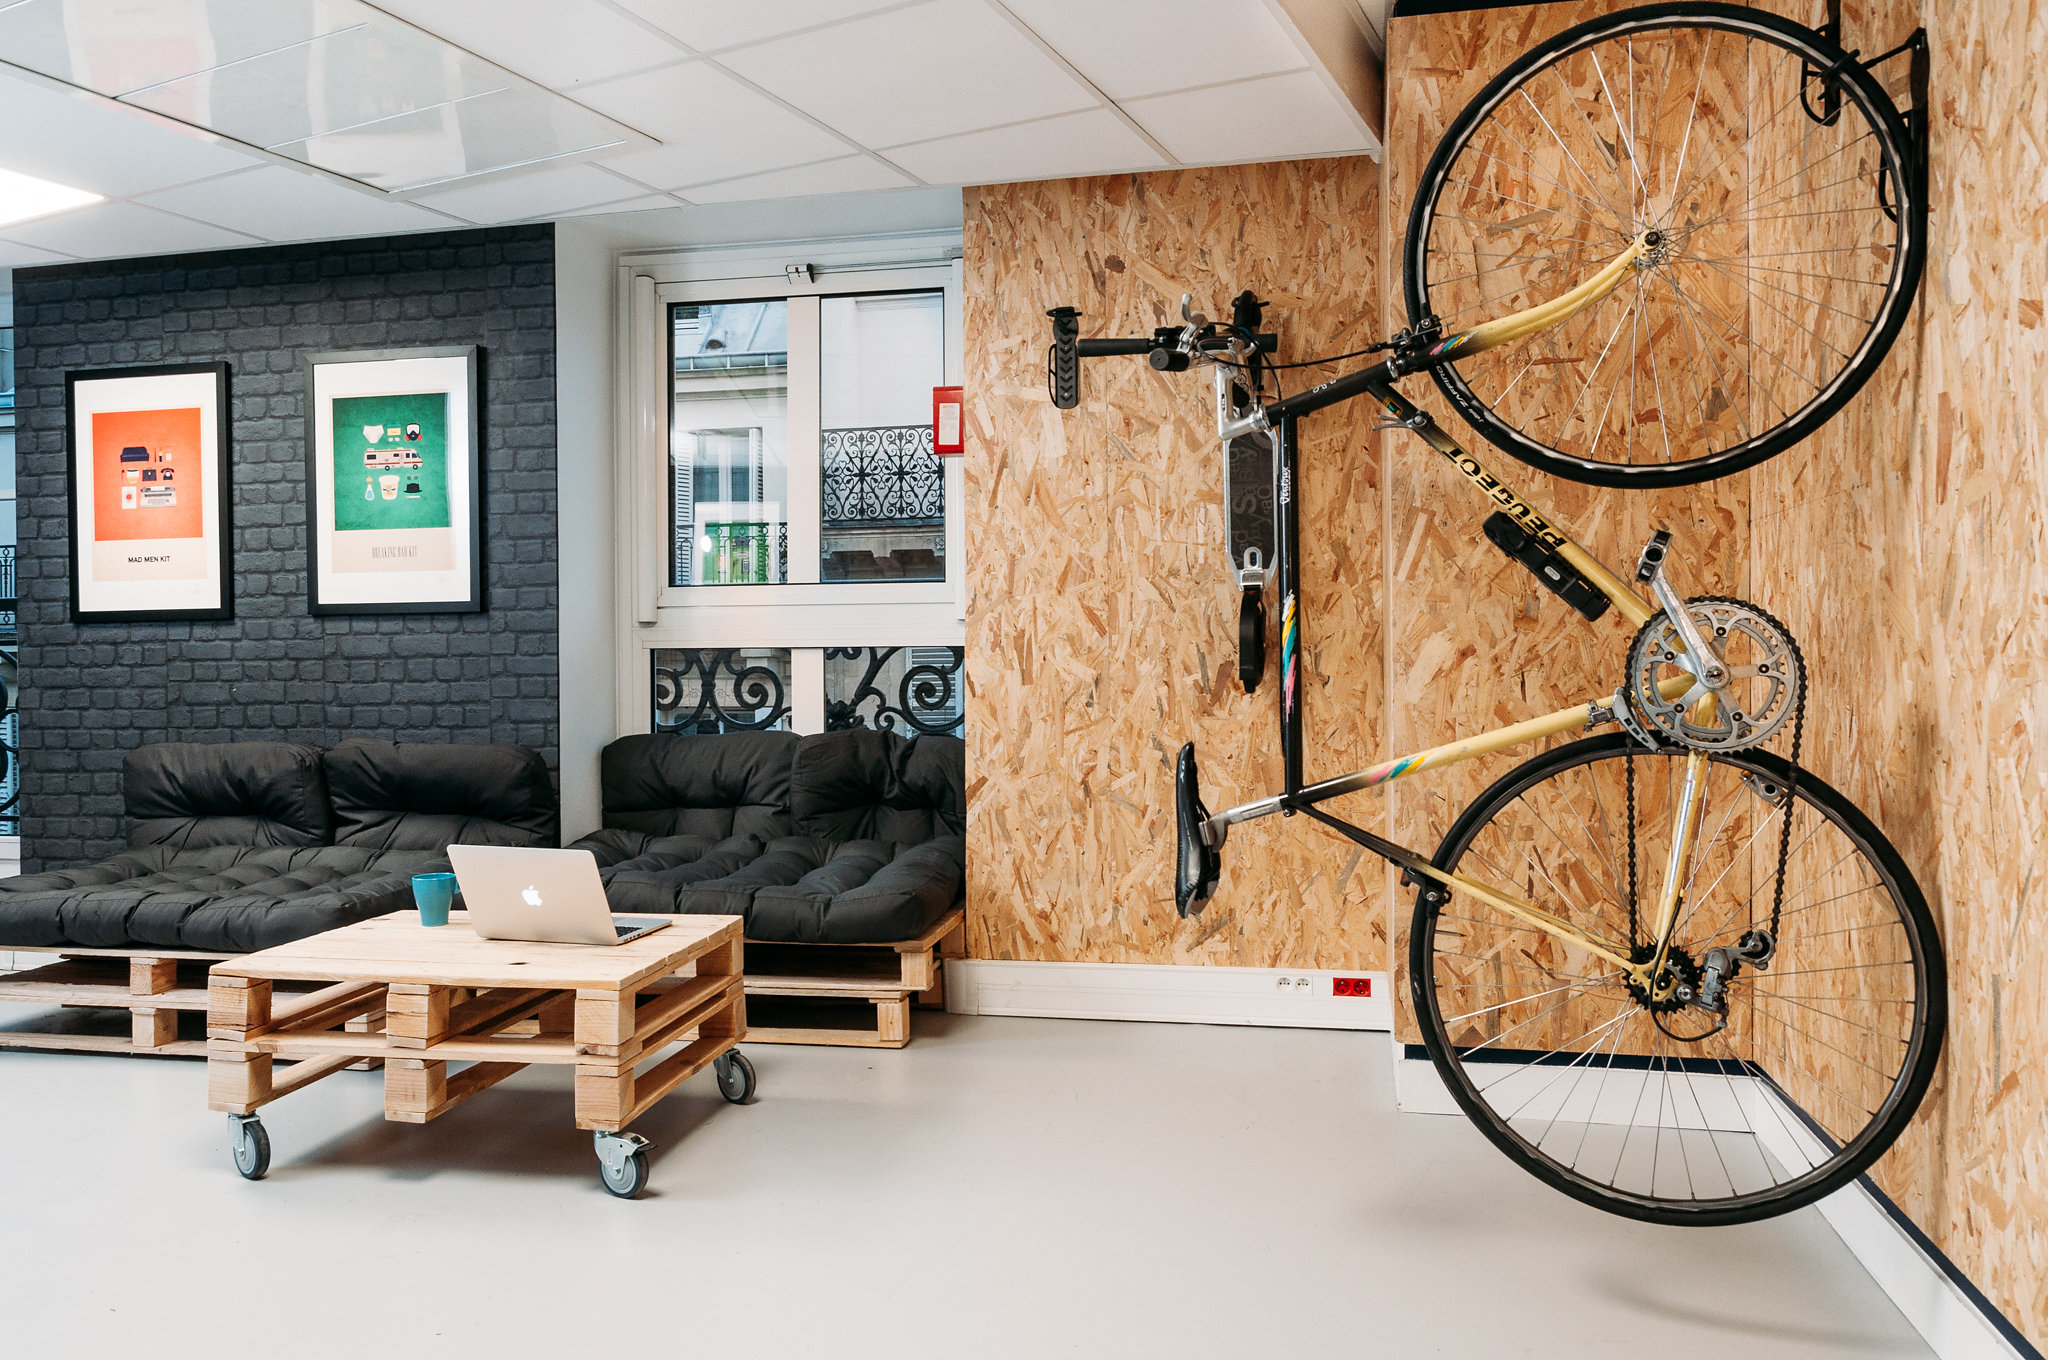
\includegraphics[width=\textwidth]{../assets/officelovin.jpg}
  \caption{Paris office of Algolia~\cite{officelovin}}
  \label{figure:algolia-office}
\end{figure}

In the other parts of the office there are couches and other places where you can work away from a desk.

% subsubsection the_office (end)
